Die API basiert hauptsächlich auf dem Framework Microsoft.EntityFrameworkCore.
Einen IHost (Host) mit einer IConfiguration (Konfiguration) schafft die Grundlage der API.
Welche API-Controller eingebunden sind, die Anbindung der Datenbank sowie die Definierung der Zugriffsrechte sind Informationen, die in der Konfiguration enthalten sind.

Das bereits im Framework eingebaute SwaggerUI kann verwendet werden, um den Aufbau der API grafisch darzustellen und Anfragen direkt über den Browser stellen zu können.
Hier werden auch Definitionen, Kommentare und Datentypen beschrieben und wie sie in der API verwendet werden können.
\linebreak

Das Verwendete Datenbanksystem ist SQLite.
Benutzer und Anwendungsdaten werden in zwei getrennten .db-Dateien gespeichert.
Der Grund für diese Wahl ist in der Funktionsweise der Anbindung begründet.
Während für die Datenbank mit den Anwendungsdaten ein Klasse vom Typ DbContext verwendet wird, benötigt die Verarbeitung der Benutzer und Rollen einen IdentityDbContext.

Damit es hier nicht zu Migrationsproblemen kommt und bei einer Änderung der Datenstruktur die Benutzerdaten nicht erneut generiert werden müssen wurden die beiden Kontext-Klassen nicht zusammengelegt.
Außerdem macht diese Methode es möglich, Anwendungsdaten und Benutzerdaten an getrennten Orten aufzubewahren, was im Sinne der Datensicherheit und des Datenschutzes ist.

Die Klassen für Benutzer- und Rollendaten werden von den Frameworks Microsoft.AspNetCore.Identity und Microsoft.AspNetCore.Identity.EntityFrameworkCore bereitgestellt. Die Eigenschaften und Beziehungen der Anwendungsdaten können Abbildung \vref{data-erm} entnommen werden.

\begin{figure}[ht]
	\centering
	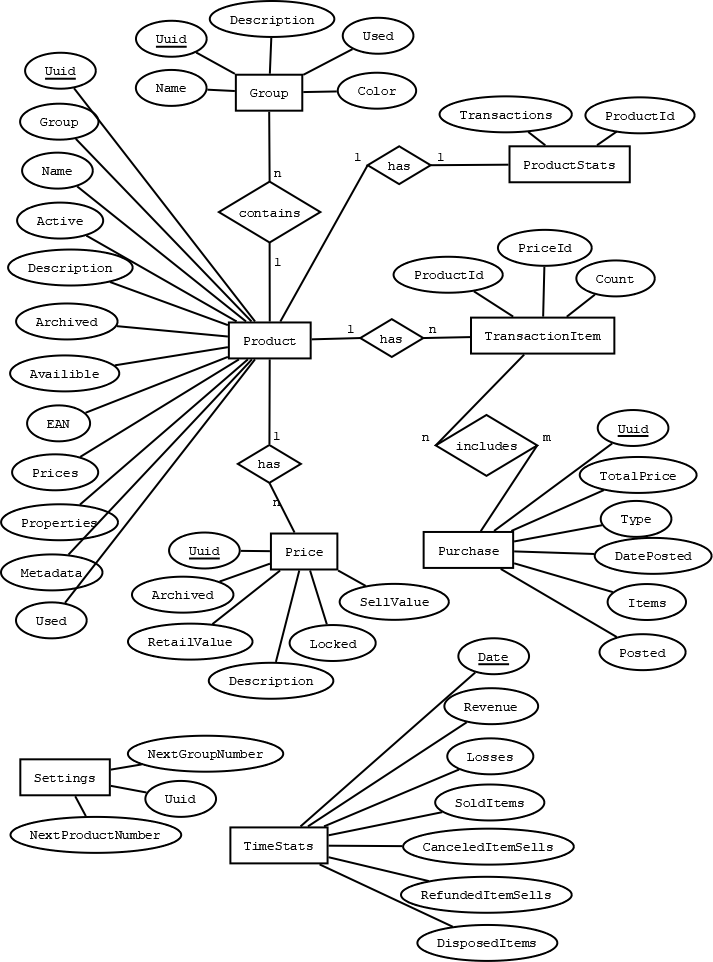
\includegraphics[width=1\linewidth]{ERM.png}
	\caption{ERM der Anwendungsdaten}
	\label{data-erm}
\end{figure}

Damit Endpunkte verwendet werden können, muss sich der Benutzer dafür authentifizieren. Dieser Vorgang kann in Abbildung \vref{login-struct} betrachtet werden.

\begin{figure}[ht]
	\centering
	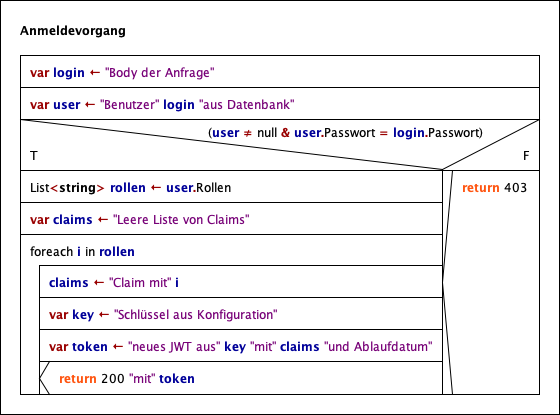
\includegraphics[width=0.7\linewidth]{Anmeldevorgang.png}
	\caption{Ablauf der Anmeldung}
	\label{login-struct}
\end{figure}